%# -*- coding: utf-8 -*-
% !TEX encoding = UTF-8 Unicode
\RequirePackage{fixltx2e}
\documentclass[aps,pre,12pt,preprint,onecolumn,showpacs,showkeys,UTF8]{revtex4-1}
\usepackage{ctex}
\usepackage{mathrsfs}
\usepackage{setspace,dcolumn}
\usepackage{subfigure}
\usepackage{graphicx,psfrag,epsfig}
\usepackage[font=small,format=plain,labelfont=bf,textfont=it,justification=raggedright,singlelinecheck=false]{caption}
\usepackage{amsmath,amsfonts,amssymb,amsthm,bm,upgreek}
\usepackage{geometry}
\usepackage[mathscr]{eucal}
\usepackage{titlesec}
\usepackage{tabularx}
\titleformat{\section}{\bf\fangsong\zihao{4}}{\thesection}{0.75em}{}
\geometry{top=2.54cm,bottom=2.54cm,left=3cm,right=3cm}
\renewcommand\appendixname{附录}
\renewcommand\abstractname{}%摘要
\renewcommand\tablename{表}
\renewcommand\figurename{图}
\makeatletter
\def\@keys@name{\songti\zihao{-4}{\bf 关键词:}}
\def\Received@name{\zihao{-5}{接收} }
\def\Revised@name{\zihao{-5}{修订} }
\def\Accepted@name{\zihao{-5}{采纳} }
\def\Published@name{\zihao{-4}{发表} }
\makeatother
\linespread{1.6}
\renewcommand{\labelenumi}{\alph{enumi}.}
\leftmargini=20mm

\begin{document}

\title{\bf\heiti\zihao{3}利用电子衍射测量Cu,Ag,Sn,Si的晶格常数\vspace{15mm}}
\author{\fangsong 乔颢\vspace{2mm}}
\affiliation{\songti\zihao{-4}北京大学物理学院2011级2班~~~~学号:1100011354 \vspace{2mm}}
\keywords{电子衍射,晶格常数,固体,指标化处理}
\email{1993422qsh@gmail.com; 18600200672}
\begin{abstract}
	\vspace{10mm}
	\begin{spacing}{1.5}
		\songti\zihao{-4}
		本实验利用马赫——曾得干涉仪制作出了复合光栅,并利用了4F相干光学处理系统配合复合光栅实现了对于图像的微分操作,验证了利用傅立叶光学进行图像处理的正确性。同时对实验制作的复合光栅进行了定量的测量得到其空间频率为$73.5mm^{-1}$以及莫尔条纹的空间频率为$2.98mm^{-1}$。
	\end{spacing}
\end{abstract}

\maketitle

\section{引言}
在普朗克和爱因斯坦关于光的微粒性理论成功的基础上,德布罗意在1924年提出了微观粒子也具有波粒二相性的假说,即对于具有能量E的微观粒子,其也具有波动的性质,其波长和频率$\mu$的关系与光波类似,可以得到其波长为:
\begin{equation}
	\lambda=\frac{h}{p}=\frac{h}{\sqrt{2meV}}
\end{equation}

而在1927年戴维孙和革末实验了电子打在镍单晶上得到了和X光衍射一样的现象。这次实验证明了德布罗意的假设,为量子力学打下了基础,同时也建立起来了一种研究物质性质的方法即为电子衍射。

相对于X光而言,电子束可以达到很高的加速速度,从而使得波长变得很短,能更好的观察到衍射角。这样能够更方便的研究晶体的几何关系。同时由于电子在物质中的穿透深度很小,所以其更适用于研究微晶,表面和薄膜的晶体结构。对于低能的电子,样品只有表面的几层电子对衍射图像有贡献,所以低能电子已经成为表面结构分析的重要手段。

透射电子显微镜(TEM)通过电子光学的手段对电子加速,聚焦并使其轰击带测样品,得到带测样品的衍射图样。本次实验就是使用透射电子显微镜观察并测定铜,银,锡,硅的电子衍射图样,并由此计算出其对应的晶格常数。这个实验的目的是要求掌握电子衍射的运动学理论,并用其研究单晶体和多晶体的衍射现象。

\section{实验}
\subsection{实验装置}
\begin{enumerate}
	\item 透射电子显微镜。\\透射电子显微镜由顶端灯丝和电子枪产生并加速电子形成电子束,通过磁透镜(利用环形磁场对电子束进行约束聚焦,功能上类似于透镜对于光的作用)的调整打入带测样品,并经过物镜目镜的放大以及光阑的约束等等成像到屏幕上并由荧光装置现实出来。其整体结构复杂,并且需要工作在基本真空的环境下以避免空气中的灰尘对于电子束的影响等。所以透射电子显微镜是一套极其复杂的大型仪器。
	\item 透射电镜辅助系统。\\ 因为透射电子显微镜工作需要许多复杂的条件,所以有一整套辅助系统对电镜提供支持。主要有提供电流的高压直流电源,市电稳压模块。提供真空的扩散泵和为扩散泵提供低压的真空泵。以及维持系统和磁透镜稳定性的散热系统等。本实验中的电镜处于常年工作状态,所以其也有一定的后备电源系统等。
	\item 透射电镜控制台。\\控制台为操作人员提供了方便快捷的操作体验,简化了原来十分复杂的调整操作。同时其也承担着协调各个系统之间的关系的作用,例如当真空度不足时就不会为灯丝加上电流以防其烧坏,当外部真空泵失效的时候会停止扩散泵的工作防止其被压强差损坏等等。同时控制台也提供了照相或者CCD的一系列设备以提供数据的采集。本电镜是使用的照相的方法收集数据。
	\item 样品。\\本实验的样品是使用真空蒸镀的方法将金属蒸镀到含孔的网上,只有足够薄的样品才不会影响到电子的通透性所以样品需要足够的薄。对于硅(Si)则是观察的纯度很高的单晶硅的边缘部分(边缘采用特殊工艺刻蚀出来,十分的薄)。
	\item 暗室等。\\提供胶片的冲洗流程。
\end{enumerate}

\subsection{实验步骤}

将样品装入样品台并将其插入电镜,等待真空度达标后打开灯丝,发射160keV的电子束,调整透镜的放大倍数为最低,移动样品台,使得电子书打在样品上。调整电子束的位置使得亮度合适并且光斑中心在屏幕的正中。调整聚焦使得像清晰。随后逐步增加放大倍数并且调整样品位置,光斑位置,光斑大小,聚焦。直至放大倍数为10万倍,这时候应该能看到清晰的样品的结构。

将电镜的工作模式切换到衍射模式,同时调整亮度以及聚焦使得到一张清晰同时亮度适中的衍射图像。



\section{数据分析及讨论}

带入公式计算可以得到光栅的周期频率有:
$$d=\frac{\lambda}{\sin{\theta}}\approx\frac{\lambda}{\theta}=\frac{dl}{\Delta x}=73.5 mm^{-1}$$

对于莫尔条纹进行拟合可以得到:

\begin{figure}[h]
	\begin{center}
		\includegraphics[width=0.8\textwidth]{pic6.eps}
		\caption{\label{fig:exp3}莫尔条纹间距拟合图像。图像表示再出现第i个微分图像时候符合光栅的水平位置}
	\end{center}
\end{figure}
\newpage
可以看出来其线性程度非常的高,计算可以得到空间频率$\nu=\frac{1}{b}=2.98 \pm 0.02 mm^{-1}$

对于图像微分的瑕疵,应该是由于光学器件并不是十分的干净,这个在移动复合光栅的时候可以明显的观测的像平面上有不规则的图样随之移动。同时因为光栅是振幅投射性质的光栅,其对于衍射条纹的衰减是十分明显的,也就显得一级衍射条纹十分的暗淡,不易观测到。再加上物并不是毛玻璃而是平行光经过光阑,光强十分的大,自身图样会因为衍射而形成光晕使得观察更不容易,综合起来导致了图像微分的效果不是十分的优良。

\section{结论}

这次实验利用马赫——曾得干涉仪制作出了复合光栅,并配合4F系统进行了光学图像的微分系统的实验,得到了预期的结果,验证了利用复合光栅可以实现光学图像微分的结论。并对制作出来的复合光栅进行了一定的测量。得到其周期间距为:
$$\nu=73.5mm^{-1}$$
以及摩尔条纹的周期为:
$$\Delta\nu=2.98 \pm 0.02 mm^{-1}$$。

 
\section{致谢}
感谢赵子强老师的指导,以及贾春燕,冉书能老师的技术支持。



\begin{thebibliography}{}
	\bibitem{Book} 吴思成,王祖铨~2010 近代物理实验(第三版)(北京:高等教育出版社)第371页.
	\bibitem{Book2} 宋菲君,陈树源~近代光学信息处理 (北京大学出版社) 
%
%
\end{thebibliography}

\clearpage
\appendix
\section{思考题}

	1、正弦光栅相对于普通光栅的优良之处也正是在于他的衍射只有1级衍射图样。所以判断正弦光线与否只需要将其放在分光计上,观察其是否有二级衍射条纹即可。不是正弦光栅的原因很有可能是因为过曝光,或者曝光不足导致的,即显影后的透射率并不和照射光强成正比。

	2、光栅空间频率加倍,$70mm^{-1}$的光栅的时候对应的应该是$4.4\times10^{-2}$的角度,加倍后可知其偏转角度也增加一倍,所以观测到的衍射条纹还在孔径范围内,不过其衍射图像会明显变暗。

	3、这样的话能够保证两次曝光的正弦光栅的空间指向是一致的而不是有夹角。不平行的话两个正弦形式的光栅就有一定的角度相互叠加使得制成的复合光栅的效果很差。

\end{document} 
